\section{Methods -- Experiment 2: Importance of Video Elements}
\label{method-2}
The first experiment showed that QV aligned closer to the participants' approximated true preferences compared to the Likert survey when choosing among a set of societal issues. To strengthen our results and examine the generalizability of QV, we designed a second experiment with three changes: (1) a change in topic domain, (2) a change in the relationship of options on the survey, (3) a change in the tangibility of the survey outcome. We describe these changes below.

First, we changed the application domain from public policy to HCI to explore if QV's advantage of better alignment to people's preferences generalizes to a different domain. HCI studies often rely on eliciting preferences from users to inform designs that involve trade-offs and in turn create better user experiences. These characteristics made HCI studies an excellent domain to test out QV. 

Second, we changed the \textit{relationships and interactions} among items in the survey. In experiment one, the different societal causes (items) impacted the society (topic) on their own without influencing each other. But experiment two focused on ballot items that represented different \textit{aspects} that jointly contributed to the same subject matter and may interact with one another, a typical case in the HCI domain. To give an analogy: the first experiment asked about preferences among chocolate, strawberry, and vanilla ice cream (paralleled options), whereas the second experiment asked about the texture, flavor, and ingredients of ice cream (aspects of the same object that may influence each other). Since relationships and dependencies may impact how users make trade-offs, we want to examine if the results from QV also align better with people's true preferences than Likert in this use case.
% We hypothesize that the latter case is more challenging for the participants to express accurately. Thus, if QV could outperform Likert in such cases, it will broaden the use cases for QV.

Lastly, the second experiment focused on a setting that surveyed matters with a more tangible and immediate outcome to the participants, a common scenario in HCI studies, as opposed to matters with a more abstract and further-in-the-future impact. This difference may also impact the relative performance of QV and Likert. 
% Our last change made the second experiment a within-subject study to understand how the same individual's expression differs using different survey tools.

We hypothesized that QV would outperform Likert in accurately representing the participants' true preferences in the new setting. To verify our hypothesis, we designed a within-subject study that elicited participants' preferences on different video elements using QV, Likert, and a pricing task. In this section, we first explain how we selected video streaming experience as the HCI study scenario. Then, we demonstrate the experiment workflow accompanied by the interfaces of the experiment. Finally, we explained the analysis approach.

%<---------------------------->%
% HCI Experiment background
%% Video HCI experiments
%% Selection of the five elements and their definitions
%% The goal of this HCI experiment is to find elements that impact participants most.
%<---------------------------->%
 
\subsection{Choice of HCI study}
The selected HCI study scenario needs to align with the three changes specified above. We set out to find a typical use case where UX/UI researchers survey users to understand what features to prioritize. In the end, we decided to use the research scenario of understanding users' preferences among various video and audio elements under network or monetary constraints \cite{molnar2013comedy, oeldorf2012bad}.
% On the one hand, we wanted to avoid creating an entirely new HCI study that required sophisticated verification. On the other hand, reproducing a prior HCI study that used Likert surveys can be costly and difficult because of the limited access to the devices, designs, or interfaces used in the study. Therefore, we developed new research based on prior research but with a new research question and study design to maintain ecological validity.

Research on video and audio elements of video playback from the lens of HCI is relatively mature. Among a variety of topics, understanding how users with bandwidth constraints made trade-offs across multiple videos and audio elements \cite{molnar2013comedy, oeldorf2012bad} is a typical topic to explore which of the $K$ aspects of the same subject should be prioritized under constraints. \textcite{oeldorf2012bad}, for example, conducted a study to examine the differences in participants' perceptions between three video bit rates, three video frame rates, and two audio sampling rates across three types of video content via a 5-point Likert scale. 
% Participants rated the overall quality, video quality, audio quality, and enjoyment level  in each condition. The study derived the conclusions from analyzing the means and standard deviations of the Likert survey results. This HCI experiment is a typical study to explore which one or some of the $K$ elements to prioritize under constraints.
% Researchers provided insights to topics including multi-media conferencing \cite{watson1996evaluating}, video-audio perception \cite{chen2006cognitive, molnar2015assessing}, and, more specifically, trade-offs among various video and audio elements under network or monetary constraints \cite{molnar2013comedy, oeldorf2012bad}. understand how users with bandwidth constraints made trade-offs covering a broad set of elements across multiple videos and audio elements. They 

We proposed a similar user research topic as in \textcite{oeldorf2012bad}'s study. We designed the experiment to answer the following question: ``Given a video with unsatisfying quality, under limited bandwidth, how should the bandwidth be allocated to enhance the five video and audio elements, including motion smoothness \cite{huynh2008temporal}, audio stability \cite{hardman1998successful}, audio quality \cite{knoche2008low}, video resolution \cite{knoche2005can}, and audio-video synchronization \cite{steinmetz1996human}, to obtain an acceptable video streaming experience from the viewers' perspective?'' We selected the five video elements based on prior work. For their detailed definitions, please refer to \Cref{elem_def}. To our knowledge, no prior work has studies the combination of five elements in a single experiment.

Prior work suggested that the type of video affected users' perceptions for video elements. In this experiment, we used a 90-second weather forecast video for the United States. There are two reasons why we chose the weather forecast video. First, the concept of a weather forecast is generic and universal. The terms used in the weather forecast are usually easy to understand. Second, since we are studying both audio and video elements, we wanted a video that conveyed information via both visuals and speech. In a weather forecast video, the meteorologist usually spoke aloud the weather while pointing at visual cues such as icons and numbers.
% There is no prior literature that looked at five combinations in a single experiment and studied them together, to the best of our knowledge. Hence, this is a valid HCI-related research question. We are also aware that these video elements' importance relies heavily on the type of video being served. 
% Video clips such as sports can contain specific jargon, while movie clips can be unfamiliar to some and not to others. a large amount of visualization but also provided information through speech. Drama and talk shows, for example, would lean towards visual elements or audio elements. Finally, visual and audio elements in a weather forecast complement each other. 

In the next section, we describe how we conducted the video elements trade-off experiment to compare the performance between Likert and QV surveys in truthfully reflecting users' preferences across the video/audio elements.
% answering the research question in identifying the video/audio elements that impact participants' streaming experience the most.

\begin{figure}[htpb]
    \centering
    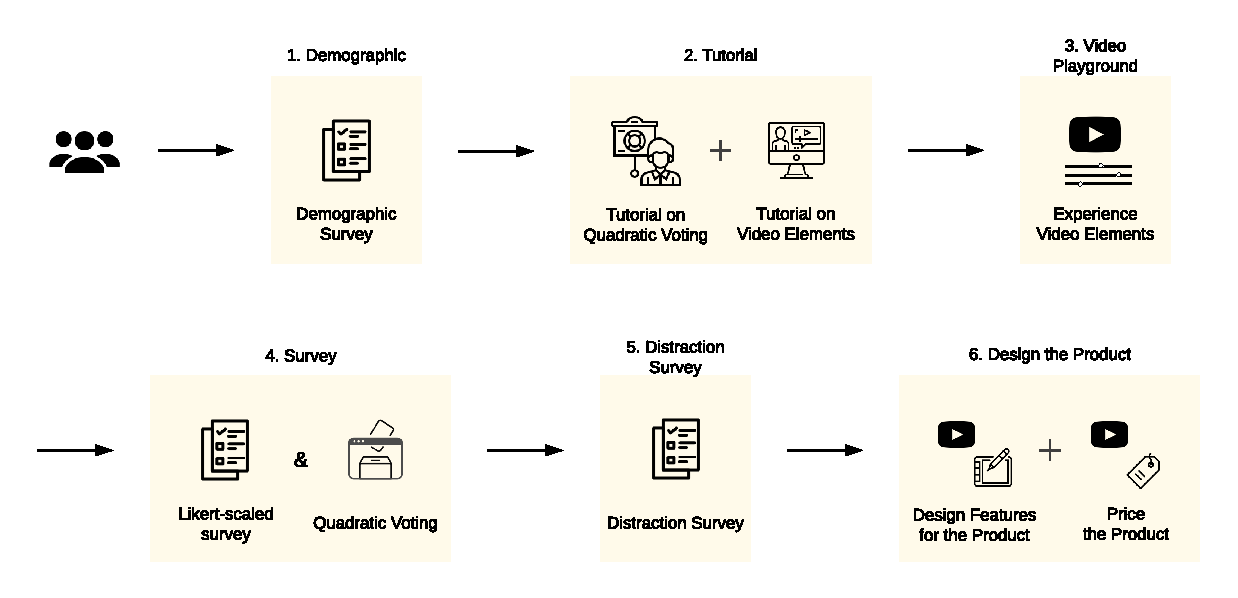
\includegraphics[width=\textwidth, keepaspectratio=true]{content/image/exp2_procedure.pdf}
    \caption{
        We used a within-subject design for experiment two. We randomly assigned participants into two groups: one group would complete the Likert survey first and then quadratic voting; the other group experienced them in a reversed order.
    }
    \label{fig:exp2_flow}
\end{figure}

\subsection{Experimental Flow}
We recruited participants on Mechanical Turk through the CloudResearch platform \cite{litman2017turkprime}. Like our first experiment, we used a pre-survey to match the participants' distribution with the U.S. population in age and education based on 2018 US census estimates. The average completion time was 35 minutes 42 seconds and all participants received \$6 as base pay and a bonus up to \$2. All participants followed six steps, as shown in \Cref{fig:exp2_flow}. The six steps were (1) demographic survey, (2) tutorials and attention checks, (3) a video playground, (4) Likert and QV surveys, (5) a distraction survey, and (6) a design task. The experiment took X minutes to complete on average. Turkers received a compensation of \$6 given quality completions and a bonus up to \$2. Now we explain the six steps in detail. We provide the experiment protocol as supplementary materials.

\subsubsection{Step 1. Demographic Survey}
We greeted participants with a consent form. In the consent form, we presented the goal of the study as understanding how people think about the importance of the different elements during video streaming. We did not reveal to the participants that this experiment aimed to compare Likert and QV until they completed the survey. Once participants gave their consent, they would fill out a demographic survey that contained questions identical to those in the first experiment.

\subsubsection{Step 2. Tutorials and Attention Checks}
In step two, we provided two tutorials to the participants. All participants would first read through a tutorial that defined the five video elements used in the experiment, via textual explanation and pairs of video examples. On the next page, they needed to answer five multiple-choice questions about the definitions of video elements and two attention checks designed to see if audio and video played fine on the participant's device. Participants would be disqualified from the experiment immediately if they answered two or more of the questions incorrectly. This step made sure participants fully understood the terminologies used in the rest of the experiment.
% In this tutorial, for each video element, we showed a pair of videos side-by-side for participants to compare how the same video would differ if a particular element were perfect and when the element is of lousy quality. 

Participants would then move on to a tutorial on how QV works, with a short instructional video supplemented with text. Participants may play with a QV interface similar to that in \Cref{fig:qv_donation}. Once the participants were confident that they understood QV, they needed to complete the same QV quiz in experiment 1. The system would disqualify the participants immediately if they answered two or more questions incorrectly.

\begin{figure}[htpb]
    \centering
    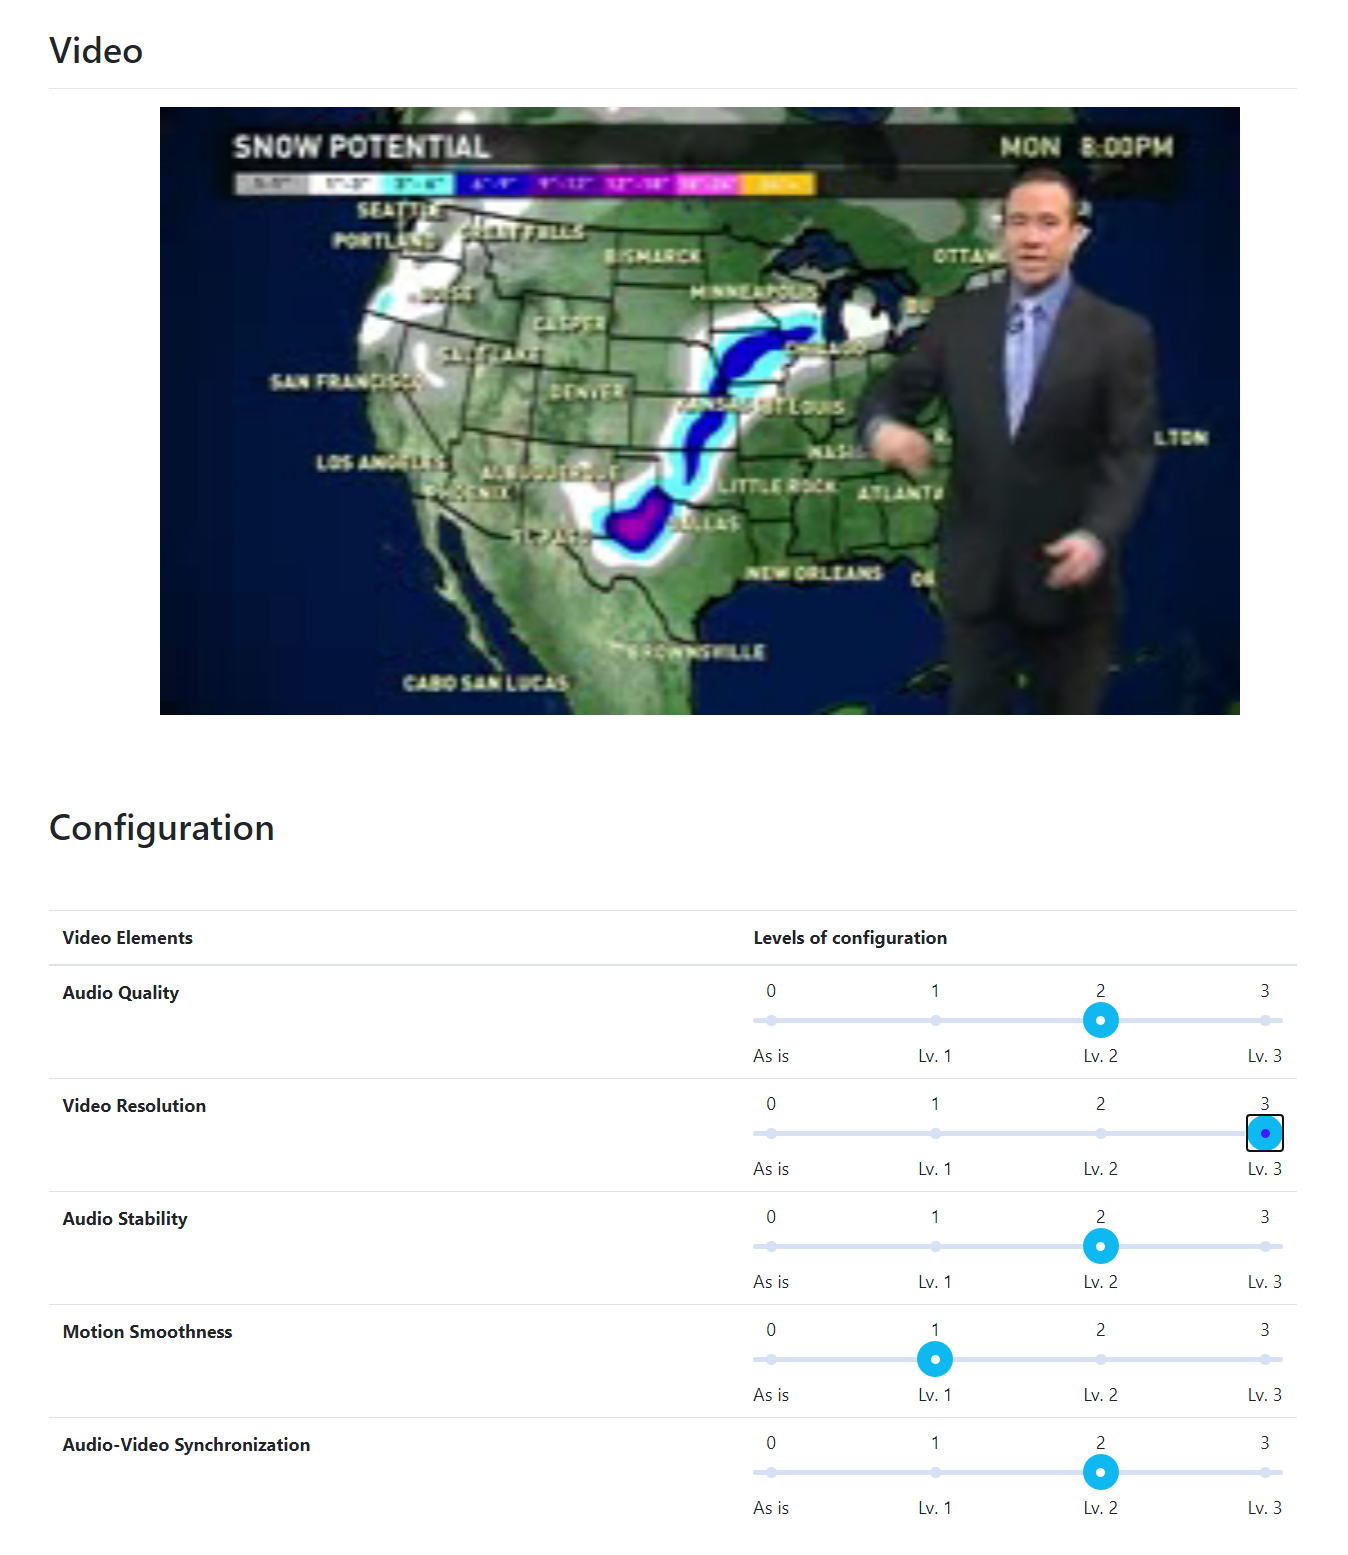
\includegraphics[width=0.8\textwidth, keepaspectratio=true]{content/image/video_playground.png}
    \caption{
        The real-time video element interface allows participants to adjust video playback elements and understand how differences in the elements impact their viewing experience. We selected four levels of quality settings for each element according to prior research, ranging from an unacceptable quality to a good quality. The technical details of this implementation are included in the appendix.
    }
    \label{fig:exp2_playground}
\end{figure}


\subsubsection{Step 3. Video Playground}
To increase this experiment's fidelity, we framed the study as a market research initiative by a fictional company (participants were not aware that the company was fictional), with a goal of providing a video-streaming product in cars using satellite-based Internet. We first showed the participants the ``current prototype" of the company's streaming service, which simulated what a weather forecast video played under limited bandwidth would look like, with all five elements at the worst quality in the range we designed to study\footnote{Motion smoothness: 32\% packet loss rate; Audio stability: 32\% packet loss rate; Video resolution: 210x280; Audio quality: 8kHz sampling rate; Audio-video synchronization: audio plays 2250ms ahead of the video}. 
% After experiencing the current prototype, the participants moved on to the next page.

To help participants better understand the impact of various enhancement levels for each element on the current prototype, we led them to a video playground shown in Fig \ref{fig:exp2_playground}. This playground allowed participants to use the control panel to adjust the levels of enhancements for all five video elements and see real-time changes in the video on the top of the page based on the updated combination of quality levels. Participants could pause and play the video at any time, and replay the video as many times as they like. We encouraged participants to test out different combinations freely in this playground and hoped they would understand the impact of each element and how the five elements interact with each other through this experience. We asked participants to describe how changing the elements impacted their experience in a free-form text question to make sure participants did experience different settings.
% It is important to note that this interface is important because we asked participants to elicit preferences among the different \textit{perspectives} of the same subject matter. Each of these perspectives might not be independent of one another.
% We then instructed them to explore how various enhancement levels on different elements in the current prototype would improve their viewing experience. 

% This interface showcased a weather forecast video on the top of the page. 
% Participants can toggle any of these five elements to any of the four levels at any time. According to the quality levels the participants set, the video playback will immediately apply those changes. We .

For each element, we provided a slider with four levels, Level 0 at the lowest quality and Level 4 at the highest. We designed the intermediate levels based on prior research such that the changes between each level of an element had a quasi-linear impact on viewers' perception. The four levels of the five video elements are listed below, from Level 0 to Level 3:
\begin{itemize}
    %20\%, 8\%, 4\%, and 0\%
    \item Motion Smoothness \cite{huynh2008temporal}: 2.5 fps, 6.25 fps, 8 fps, and 25 fps
    %20\%, 8\%, 4\%, and 0\%
    \item Audio Stability \cite{hardman1998successful}: 20\%, 10\%, 5\%, and 0\% probability in packet loss
    %210x280, 294x392, 364x486, and 420x560     
    \item Video Resolution \cite{knoche2005can}: 120x90 at 32K bit rate, 168x126 at 64K bit rate, 240x180 at 96K bit rate, and 240x180 at 224K bit rate all encoded using the wmv2 (Windows Media Video 8) codec 
    %8kHz, 11kHz, 16kHz, and 48kHz 
    \item Audio Quality \cite{knoche2008low, noll1993wideband}: 8kHz, 16kHz, 24kHz, 32kHz encoded using the aac (Advanced Audio Coding) codec
    %1850, 1615, 1050, or 0 ms ahead
    \item Audio-Video Synchronization \cite{steinmetz1996human}: 2000ms, 1250ms,  750ms or 0ms
\end{itemize}



\subsubsection{Step 4. Surveying Preferences}
After experiencing how different enhancements on the five video elements impacted their viewing experience, we collected participants' opinions on how critical the improvements on each video element in the current prototype were for them to understand the weather forecast video. Participants completed a Likert survey and a QV survey in a randomized order to prevent ordering effect. Since this was a within-subject study, we randomized the display order of the elements on the surveys to minimize carryover effect and ordering effect. The QV interface was similar to that in experiment 1. We designed the credit budget to be 100 voice credits, the best option based on experiment one, i.e., $N^2 x O$, where $N=5$ and $O=4$ in this case.

\subsubsection{Step 5. Distraction Survey}
Before moving on to the task for eliciting the participant's truthful preference as approximated ground truth, we designed a distraction survey that asked about participants' consumption preferences across different subscription tiers for several well-known streaming services. This survey aimed to prevent participants from translating their survey responses directly to the next task. We told participants that this survey results would be used in an important part for the next task.

\subsubsection{Step 6. Design a Product}
To capture a participant's truthful preferences on how much they \textit{value} each of the five video elements, we created a ``Design a Product'' task. To create a high fidelity scenario, we told participants that the system assigned them into the designer group, and their job was to design a streaming service for cars via satellite internet. Their goal was to design and price their product such that another participant (fictional but the participants were not aware), similar to them based on demographic information and the consumption preference survey from the buyer group, would be willing to purchase the product. We emphasized that their product should be affordable and should allow the buyer to understand the weather forecast video. To incentivize the participants, we offered them 10\% of the final price they proposed as their bonus if the buyer decided to purchase their product.

% The instruction also told participants to consider that each element is associated with a cost, and the buyer will need to pay each element's cost. We told participants that if the buyer decides to purchase the product, they will receive 10\% of the final price they proposed as their commission. 

We guided participants to complete the task in two steps. \Cref{fig:exp2_store} shows the two interfaces. In the first step, participants needed to select one of the two qualities for each video element, a lower quality and a higher quality, and ``assemble'' the product. Quality one refers to level 0 in the playground, the worst one they had experienced. For quality two, we selected the quality levels in the playground that matched what prior research showed to be the ``acceptable level''\footnote{Place the five quality two values here}. Participants could see real-time changes to the video as they updated the qualities. Participants were essentially making a binary decision of whether a video element was ``important'' or ``not important'' for them, and equivalently for the buyer that had similar preferences as them. 
% This binary design prevents us from bounding participants' choices when provided a slider. 

In the second step, participants set a price they thought to be reasonable for each of the five elements between \$0 - \$4 based on the qualities they selected and how much they thought the buyer would value them. The sum of these prices was the total price of the product. We reminded participants throughout the task that the higher they priced the elements, the more their bonus could be. However, if they overpriced any element from the buyer's perspective, the buyer might not purchase their design and they would fail to gain any bonus. 

The goal of this design was to elicit the truthful willingness-to-pay for each participant as the approximated ground truth of their preferences. Our set-up was incentive-compatible and the best strategy for the participants was to price based on how they themselves valued each of the elements. If they priced the product higher than their accurate valuations, the ``buyer'' with similar demographic and consumption preferences as them would reject their proposal, given that the buyer would likely value the elements the same way. Vice versa, if the participants set their prices to be lower than their actual willingness-to-pay, they would lose out on earning a higher bonus.

\begin{figure}[htpb]
    \centering
    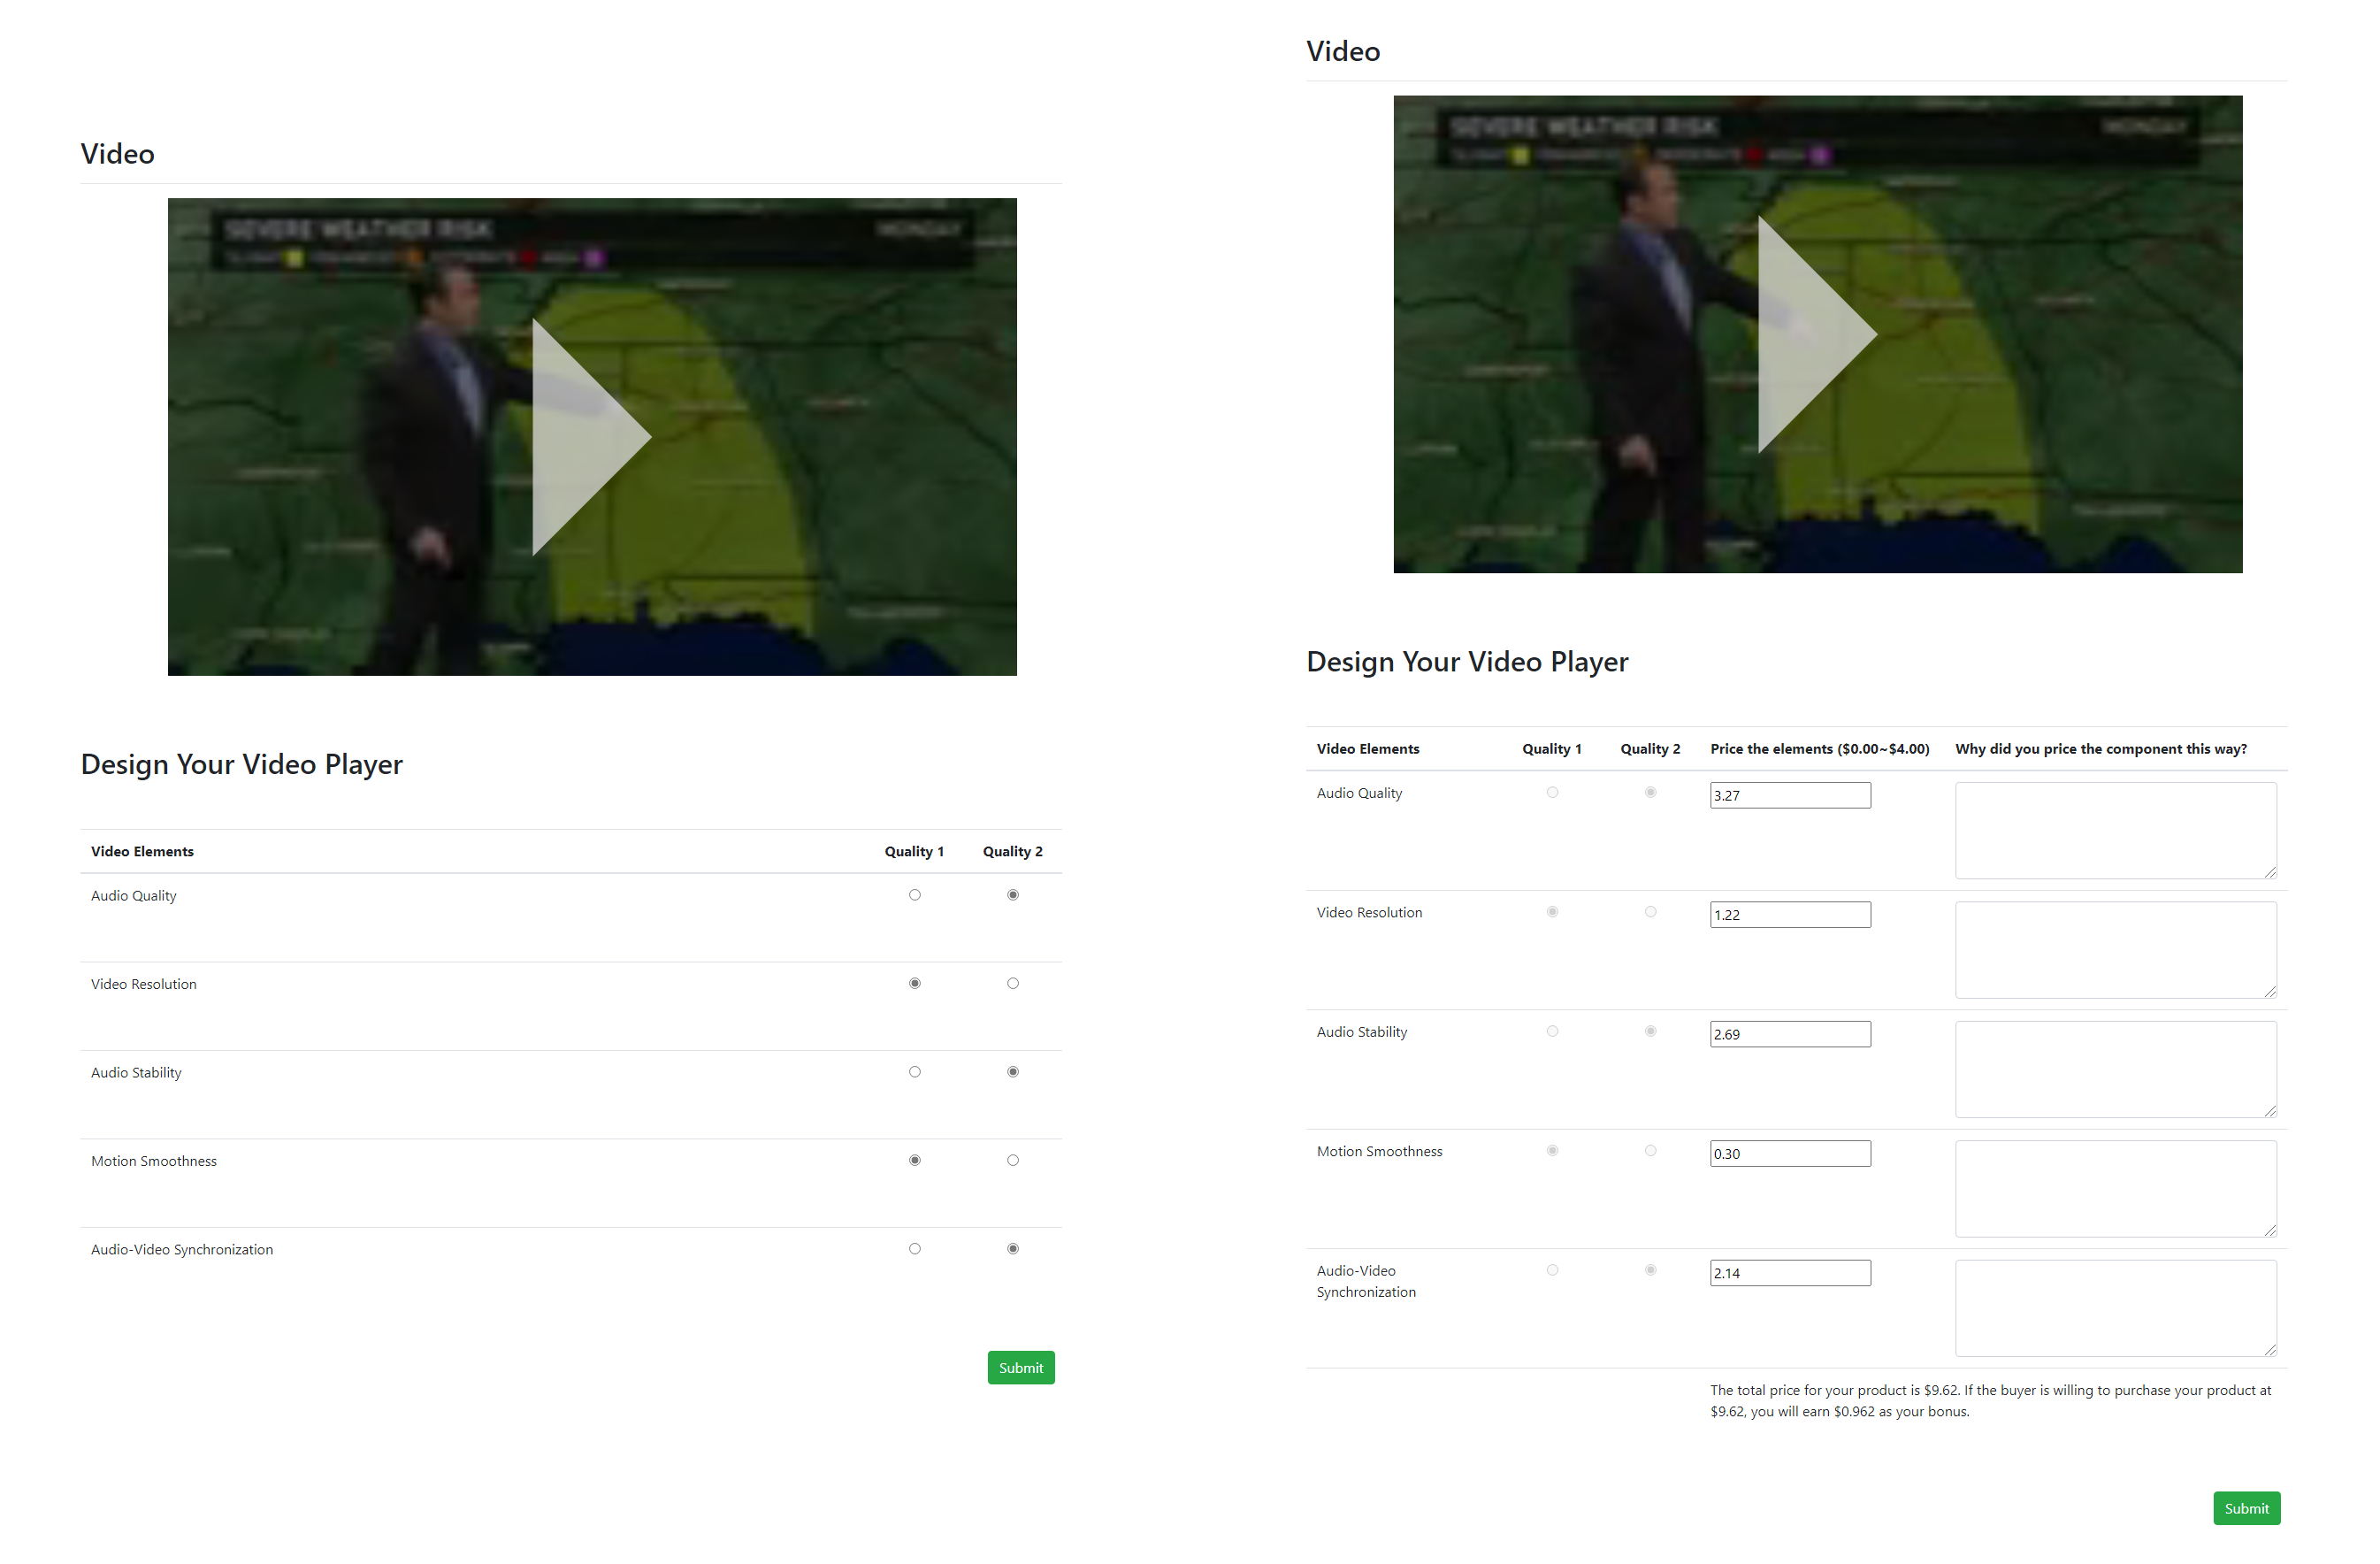
\includegraphics[width=\textwidth, keepaspectratio=true]{content/image/design_task.png}
    \caption{
        The two steps participants encountered when completing Step 6 of the survey. Participants would first need to select which one of the two qualities they would include in their video streaming product. Participants could see real-time changes to the video as they updated the qualities. Once they made their decisions, participants would price each of the elements bewteen \$0 and \$4. Participants would receive a commission worth 10\% of the total price if the buyer accepted their product at their set prices.
    }
    \label{fig:exp2_store}
\end{figure}

% Notice that instead of giving participants the power to select the quality over various levels as they did in the video playground in step three. We only provide two qualities for each video element. 

\subsection{System Design}
We built the system for this experiment on top of the system for experiment one. To create real-time adjustments in video qualities, we pre-generated video-only and audio-only files of different qualities. When a participant changed an audio or video quality setting, the system served the correct combination of video and audio files. We used JavaScript to adjust the video-audio synchronization in the front-end at real-time.

This design balanced the need for a high network speed to stream every configuration from the server and the need for a powerful client to compute the video and audio qualities. The experiment source code for experiment two is publicly available \footnote{Not yet public}, and so is the video interface as a stand-alone repository \footnote{https://github.com/hank0982/QV-app}. More details of the system implementation are provided in the appendix (xxx).

\subsection{Analysis Method}

Since RQ2 is also about the degree of alignment, similar to RQ1, we followed a similar analysis approach as described in \Cref{method_exp1}. In experiment 2, we compared the alignment between survey responses with the prices set in an incentive-compatible scenario. We used the same definition of ``alignment" and the same metric for alignment, Cosine similarity angle, as explained in \Cref{alignment_metric}. For the Likert group, we mapped the ordinal responses into a vector where the result for each video element ranges from $-2$ to $2$. For QV, the vector contains the number of votes for each video element. Then, we computed the Cosine similarity angle between a Likert or QV vector and the absolute prices set by the same participant,.

Once we obtained the two sets of Cosine similarity angles, one for Likert and one for QV, we applied the same Bayesian formulation to model the mean Cosine similarity angle in both groups as detailed in \Cref{exp1:The Bayesian Model}. Then, we compared the two distributions.